\documentclass[a4paper, 12pt]{article}

% packages
\usepackage{amssymb}
\usepackage[fleqn]{mathtools}
\usepackage{tikz}
\usepackage{enumerate}
\usepackage{bussproofs}
\usepackage{xcolor}
\usepackage[margin=1.3cm]{geometry}
\usepackage{logicproof}
\usepackage{diagbox}
\usepackage{listings}
\usepackage{graphicx}
\usepackage{lstautogobble}
\usepackage{hyperref}
\usepackage{multirow}
\usepackage{tipa}
\usepackage{pgfplots}
\usepackage{adjustbox}

% tikz libraries
\usetikzlibrary{
    decorations.pathreplacing,
    arrows,
    shapes,
    shapes.gates.logic.US,
    circuits.logic.US,
    calc,
    automata,
    positioning,
    intersections
}

\pgfplotsset{compat=1.16}

\pgfmathdeclarefunction{gauss}{2}{%
  \pgfmathparse{1/(#2*sqrt(2*pi))*exp(-((x-#1)^2)/(2*#2^2))}%
}

\allowdisplaybreaks % allow environments to break
\setlength\parindent{0pt} % no indent

% shorthand for verbatim
% this clashes with logicproof, so maybe fix this at some point?
\catcode`~=\active
\def~#1~{\texttt{#1}}

% code listing
\lstdefinestyle{main}{
    numberstyle=\tiny,
    breaklines=true,
    showspaces=false,
    showstringspaces=false,
    tabsize=2,
    numbers=left,
    basicstyle=\ttfamily,
    columns=fixed,
    fontadjust=true,
    basewidth=0.5em,
    autogobble,
    xleftmargin=3.0ex,
    mathescape=true
}
\newcommand{\dollar}{\mbox{\textdollar}} %
\lstset{style=main}

% augmented matrix
\makeatletter
\renewcommand*\env@matrix[1][*\c@MaxMatrixCols c]{%
\hskip -\arraycolsep
\let\@ifnextchar\new@ifnextchar
\array{#1}}
\makeatother

% ceiling / floor
\DeclarePairedDelimiter{\ceil}{\lceil}{\rceil}
\DeclarePairedDelimiter{\floor}{\lfloor}{\rfloor}

% custom commands
\newcommand{\indefint}[2]{\int #1 \, \mathrm{d}#2}
\newcommand{\defint}[4]{\int_{#1}^{#2} #3 \, \mathrm{d}#4}
\newcommand{\pdif}[2]{\frac{\partial #1}{\partial #2}}
\newcommand{\dif}[2]{\frac{\mathrm{d}#1}{\mathrm{d}#2}}
\newcommand{\limit}[2]{\raisebox{0.5ex}{\scalebox{0.8}{$\displaystyle{\lim_{#1 \to #2}}$}}}
\newcommand{\limitsup}[2]{\raisebox{0.5ex}{\scalebox{0.8}{$\displaystyle{\limsup_{#1 \to #2}}$}}}
\newcommand{\summation}[2]{\sum\limits_{#1}^{#2}}
\newcommand{\product}[2]{\prod\limits_{#1}^{#2}}
\newcommand{\intbracket}[3]{\left[#3\right]_{#1}^{#2}}
\newcommand{\laplace}{\mathcal{L}}
\newcommand{\fourier}{\mathcal{F}}
\newcommand{\mat}[1]{\boldsymbol{#1}}
\renewcommand{\vec}[1]{\boldsymbol{#1}}
\newcommand{\rowt}[1]{\begin{bmatrix}
    #1
\end{bmatrix}^\top}
\DeclareMathOperator*{\argmax}{argmax}
\DeclareMathOperator*{\argmin}{argmin}

\newcommand{\lto}[0]{\leadsto\ }

\newcommand{\ulsmash}[1]{\underline{\smash{#1}}}

\newcommand{\powerset}[0]{\wp}
\renewcommand{\emptyset}[0]{\varnothing}

\makeatletter
\newsavebox{\@brx}
\newcommand{\llangle}[1][]{\savebox{\@brx}{\(\m@th{#1\langle}\)}%
  \mathopen{\copy\@brx\kern-0.5\wd\@brx\usebox{\@brx}}}
\newcommand{\rrangle}[1][]{\savebox{\@brx}{\(\m@th{#1\rangle}\)}%
  \mathclose{\copy\@brx\kern-0.5\wd\@brx\usebox{\@brx}}}
\makeatother
\newcommand{\lla}{\llangle}
\newcommand{\rra}{\rrangle}
\newcommand{\la}{\langle}
\newcommand{\ra}{\rangle}
\newcommand{\crnr}[1]{\text{\textopencorner} #1 \text{\textcorner}}
\newcommand{\bnfsep}[0]{\ |\ }
\newcommand{\concsep}[0]{\ ||\ }

\newcommand{\axiom}[1]{\AxiomC{#1}}
\newcommand{\unary}[1]{\UnaryInfC{#1}}
\newcommand{\binary}[1]{\BinaryInfC{#1}}
\newcommand{\trinary}[1]{\TrinaryInfC{#1}}
\newcommand{\quaternary}[1]{\QuaternaryInfC{#1}}
\newcommand{\quinary}[1]{\QuinaryInfC{#1}}
\newcommand{\dproof}[0]{\DisplayProof}
\newcommand{\llabel}[1]{\LeftLabel{\scriptsize #1}}
\newcommand{\rlabel}[1]{\RightLabel{\scriptsize #1}}

\newcommand{\ttbs}{\char`\\}
\newcommand{\lrbt}[0]{\ \bullet\ }

% colours
\newcommand{\violet}[1]{\textcolor{violet}{#1}}
\newcommand{\blue}[1]{\textcolor{blue}{#1}}
\newcommand{\red}[1]{\textcolor{red}{#1}}
\newcommand{\teal}[1]{\textcolor{teal}{#1}}

% reasoning proofs
\usepackage{ltablex}
\usepackage{environ}
\keepXColumns
\NewEnviron{reasoning}{
    \begin{tabularx}{\textwidth}{rlX}
        \BODY
    \end{tabularx}
}
\newcommand{\proofline}[3]{$(#1)$ & $#2$ & \hfill #3 \smallskip \\}
\newcommand{\proofarbitrary}[1]{& take arbitrary $#1$ \smallskip \\}
\newcommand{\prooftext}[1]{\multicolumn{3}{l}{#1} \smallskip \\}
\newcommand{\proofmath}[3]{$#1$ & = $#2$ & \hfill #3 \smallskip \\}
\newcommand{\prooftherefore}[1]{& $\therefore #1$ \smallskip \\}
\newcommand{\proofbc}[0]{\prooftext{\textbf{Base Case}}}
\newcommand{\proofis}[0]{\prooftext{\textbf{Inductive Step}}}

% ER diagrams
\newcommand{\nattribute}[4]{
    \node[draw, state, inner sep=0cm, minimum size=0.2cm, label=#3:{#4}] (#1) at (#2) {};
}
\newcommand{\mattribute}[4]{
    \node[draw, state, accepting, inner sep=0cm, minimum size=0.2cm, label=#3:{#4}] (#1) at (#2) {};
}
\newcommand{\dattribute}[4]{
    \node[draw, state, dashed, inner sep=0cm, minimum size=0.2cm, label=#3:{#4}] (#1) at (#2) {};
}
\newcommand{\entity}[3]{
    \node[] (#1-c) at (#2) {#3};
    \node[inner sep=0cm] (#1-l) at ($(#1-c) + (-1, 0)$) {};
    \node[inner sep=0cm] (#1-r) at ($(#1-c) + (1, 0)$) {};
    \node[inner sep=0cm] (#1-u) at ($(#1-c) + (0, 0.5)$) {};
    \node[inner sep=0cm] (#1-d) at ($(#1-c) + (0, -0.5)$) {};
    \draw
    ($(#1-c) + (-1, 0.5)$) -- ($(#1-c) + (1, 0.5)$) -- ($(#1-c) + (1, -0.5)$) -- ($(#1-c) + (-1, -0.5)$) -- cycle;
}
\newcommand{\relationship}[3]{
    \node[] (#1-c) at (#2) {#3};
    \node[inner sep=0cm] (#1-l) at ($(#1-c) + (-1, 0)$) {};
    \node[inner sep=0cm] (#1-r) at ($(#1-c) + (1, 0)$) {};
    \node[inner sep=0cm] (#1-u) at ($(#1-c) + (0, 1)$) {};
    \node[inner sep=0cm] (#1-d) at ($(#1-c) + (0, -1)$) {};
    \draw
    ($(#1-c) + (-1, 0)$) -- ($(#1-c) + (0, 1)$) -- ($(#1-c) + (1, 0)$) -- ($(#1-c) + (0, -1)$) -- cycle;
}

% AVL Trees
\newcommand{\avltri}[4]{
    \draw ($(#1)$) -- ($(#1) + #4*(0.5, -1)$) -- ($(#1) + #4*(-0.5, -1)$) -- cycle;
    \node at ($(#1) + #4*(0, -1) + (0, 0.5)$) {#3};
    \node at ($(#1) + #4*(0, -1) + (0, -0.5)$) {#2};
}

% RB Trees
\tikzset{rbtr/.style={inner sep=2pt, circle, draw=black, fill=red}}
\tikzset{rbtb/.style={inner sep=2pt, circle, draw=black, fill=black}}

% Samples
\tikzset{spos/.style={inner sep=2pt, circle, draw=black, fill=blue!20}}
\tikzset{sneg/.style={inner sep=2pt, circle, draw=black, fill=red!20}}

% Joins
\newcommand\ljoin{\stackrel{\mathclap{\normalfont\mbox{\tiny L}}}{\bowtie}}
\newcommand\rjoin{\stackrel{\mathclap{\normalfont\mbox{\tiny R}}}{\bowtie}}
\newcommand\ojoin{\stackrel{\mathclap{\normalfont\mbox{\tiny O}}}{\bowtie}}

\setcounter{MaxMatrixCols}{100}

% actual document
\begin{document}
    {\sc Computing $3^\text{rd}$ Year Notes} \hfill ~https://github.com/lin-e/imperial-revision~
    \rule{\textwidth}{0.1pt}
    \section*{CO339 - Performance Engineering \hfill (60017)}
        \subsection*{Introduction}
            Performance is how well a person / machine does work or activity.
            However we need to define \textbf{well}, which is something that is perceived by the user of the code.
            We first assume that the software is bug-free (functional), and the perceived quality is therefore usually associated with speed of execution (treat it as end-to-end execution for now).
            \medskip

            High performance computing is usually focused on a single problem (such as fluid dynamics, weather simulation, etc).
            The problem is usually `high value', with some significant benefit, is relatively simple (narrowly scoped, however speed is difficult), and is occasionally supported by special hardware, such as GPUs or tensor processing units built to support ML workloads.
            \medskip

            However, performance engineering focuses on systems (complex, flexible pieces of software).
            Examples of systems include big data systems, DBMS, AI systems (such as \textit{Tensorflow}, \textit{Torch}, etc), as well as operating system kernels and operating system tools (such as ~awk~, ~grep~, ~sed~).
            \medskip

            A system is often made up of \textbf{components} which interact to achieve a greater goal.
            These are usually applicable to multiple problems or domains (they are generic); this differs from a well-designed application as the goal is domain-agnostic, hence they are designed to be flexible at runtime - for example, we don't want to recompile ~grep~ every time we want to search for a string.
            \medskip

            The need for flexibility arises from the fact that we do not know the exact operating conditions for a system during development.
            For example, a data management system will not know the schema beforehand (could be sensor data, or user data etc).
            Another example is an OS not knowing the number of users, \textit{Tensorflow} doesn't know the dimensionality of the data, or ~grep~ not knowing what regular expression we intend to search for.
            \medskip

            Software systems are complex and developed over years, and therefore must be maintainable.
            They also need to be fast.
            The challenge is to build a system which strikes a balance, within the classic trade-off triangle (where we choose two of the three);
            \begin{center}
                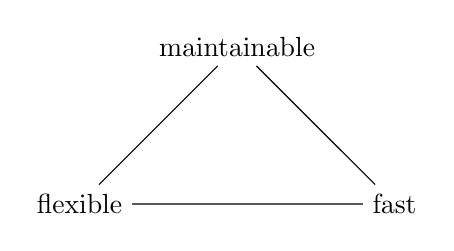
\begin{tikzpicture}
                    \node (m) at (0, 0) {maintainable};
                    \node (fl) at (-2, -2) {flexible};
                    \node (fa) at (2, -2) {fast};
                    \draw (m) -- (fl) -- (fa) -- (m);
                \end{tikzpicture}
            \end{center}
            Instead of having only flexible and fast code, we need to think about what parts should be prioritised for flexibility, what parts for speed, and what parts should be maintainable.
            \subsubsection*{Example}
                The challenge here is to count lines in a CSV file which contain the phrase ``  FAUST:'' - two spaces, followed by ~FAUST~, followed by a colon.
                This could be done with the command;
                \begin{lstlisting}
                    egrep -c '^  FAUST:$\dollar$' faust.txt
                \end{lstlisting}
                An example for this, in C++, would be as follows;
                \begin{lstlisting}
                    class Operator {
                    public:
                      virtual char const* getNextString() = 0; // abstract class
                    };

                    class ArrayReader : public Operator {
                      char const* inputArray;
                      bool isRead = false;
                    public:
                      ArrayReader(char const* array):inputArray(array){};
                      char const* getNextString() { // only return once
                        if (isRead)
                          return nullptr;

                        isRead = true;
                        return inputArray;
                      }
                    };

                    class LineSeparator : public Operator {
                      Operator&& input;
                      char const* currentString = nullptr; // string from input
                    public:
                      LineSeparator(Operator&& input):input(std::move(input)){};
                      char const* getNextString() {
                        if (currentString == nullptr)
                          currentString = input.getNextString();
                        auto result = currentString; // keep a backup
                        if (currentString != nullptr) { // we want to split this
                          // keep iterating until new line or end of string
                          while (*currentString != '\n' && *currentString != '\0')
                            currentString++

                          if (*currentString == '\n')
                            currentString++; // advance to string after
                          else if (*currentString == '\0')
                            return nullptr; // reached end of string
                        }
                        return result
                      }
                    };

                    class LineMatcher : public Operator {
                      Operator&& input;
                    public:
                      LineMatcher(Operator&& input):input(std::move(input)){};
                      char const* getNextString() {
                        for (auto candidate = input.getNextString(); candidate != nullptr; candidate = input.getNextString()) {
                          if (candidate[0] == ' ' && candidate[1] == ' ' && candidate[2] == 'F' &&
                              candidate[3] == 'A' && candidate[4] == 'U' && candidate[5] == 'S' &&
                              candidate[6] == 'T' && candidate[7] == ':' && candidate[8] == '\n')
                            return candidate;
                        }
                        return nullptr;
                      }
                    }

                    class LineCounter {
                      Operator&& input;
                    public
                      LineCounter(Operator&& input):input(std::move(input)){};
                      unsigned long getCount() {
                        auto result = 0UL;
                        for (auto inputLine = input.getNextString(); inputLine != nullptr, inputLine = input.getNextString()) {
                          result++;
                        }
                        return result;
                      }
                    }

                    int main(int argc, char *argv[]) {
                      auto fd = open(argv[1], O_RDONLY);
                      auto fileSize = lseek(fs, 0L, SEEK_END);
                      lseek(fd, 0UL, SEEK_SET); // reset to beginning
                      auto data = (char*)mmap(nullptr, fileSize, PROT_READ, MAP_SHARED, fd, 0);
                      auto result = LineCounter(LineMatcher(LineSeparator(ArrayReader(data)))).getCount();
                      printf("%lu\n", result);
                      return 0;
                    }
                \end{lstlisting}
                However, this is a significant amount slower than ~grep~.
                While this was a good implementation from an object oriented view, it's bad for performance.
                \begin{lstlisting}
                    int main(int argc, char *argv[]) {
                      auto fd = open(argv[1], O_RDONLY);
                      auto fileSize = lseek(fs, 0L, SEEK_END);
                      lseek(fd, 0UL, SEEK_SET); // reset to beginning
                      auto data = (char*)mmap(nullptr, fileSize, PROT_READ, MAP_SHARED, fd, 0);
                      auto result = 0;
                      // stop 9 chars before end
                      for (auto i =0; i < fileSize - 9; i++) {
                        if (data[i] == '\n' &&
                            data[i+1] == ' ' && data[i+2] == ' ' && data[i+3] == 'F' &&
                            data[i+4] == 'A' && data[i+5] == 'U' && data[i+6] == 'S' &&
                            data[i+7] == 'T' && data[i+8] == ':' && data[i+9] == '\n')
                          result++;
                      }

                      printf("%lu\n", result);

                      return 0;
                    }
                \end{lstlisting}
                While this code, compiled with ~-O3~ is better than the first implementation, it's still slightly slower than ~grep~.
                We can do better (only the loop this time);
                \begin{lstlisting}
                    for (auto i =0; i < fileSize - 9; i++) {
                      long word = *(long*)"  FAUST:"; // gives a bit pattern representing the string
                      if (*(long*)(data + i) == word && data[i+8] == '\n')
                        result++;
                    }
                \end{lstlisting}
                This can be compiled for native (and also gives better performance than ~grep~);
                \begin{center}
                    ~clang++ -O3 -march=native -mtune=native count.cpp~
                \end{center}
                This follows the following process, where we have an idea, make a functional solution (well designed), and then improving the performance;
                \begin{center}
                    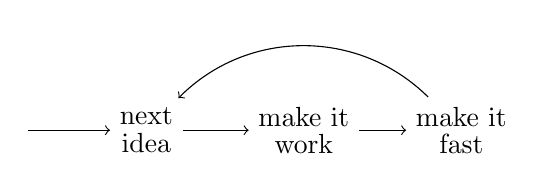
\begin{tikzpicture}
                        \node (a) at (0, 0) {\shortstack{next\\idea}};
                        \node (b) at (2, 0) {\shortstack{make it\\work}};
                        \node (c) at (4, 0) {\shortstack{make it\\fast}};
                        \draw
                        (-1.5, 0) edge[->] (a)
                        (a) edge[->] (b)
                        (b) edge[->] (c)
                        (c) edge[->, bend right=45] (a);
                    \end{tikzpicture}
                \end{center}
            \subsubsection*{Target}
                One question is to define how fast is fast enough.
                \begin{enumerate}[1.]
                    \itemsep0em
                    \item \textbf{define a target metric}
                        \begin{itemize}
                            \itemsep0em
                            \item \textbf{throughput} \hfill how many runs can be performed in a given time
                            \item \textbf{latency} \hfill trade-off with throughput (what we've been looking at)
                            \item \textbf{scalability} \hfill how well it works with more machines
                            \item \textbf{memory usage} \hfill stay within memory constraints
                            \item \textbf{energy consumption} \hfill energy related to cooling in data centres
                            \item \textbf{TCO} \hfill total ownership cost
                            \item \textbf{efficiency} \hfill work over time
                        \end{itemize}
                    \item \textbf{decide when requirements are met}
                        \smallskip

                        An easy approach to this it to set an optimisation budget (in terms of developer time / cost).
                        For example, we can ask how much a customer is willing to spend to optimise something.
                        \medskip

                        On the other hand, we can set a target, requirement, or threshold (at least this fast).
                        This might have real-time requirements; soft (if it misses the requirements, it's an error), or hard (if it misses the requirement, it's considered a failure).
                        These are often referred to as \textbf{Quality-of-Service (QoS)} objectives.
                        \medskip

                        These objectives are statistical properties of a metric that must hold for a system.
                        For example, we can put a condition for a game to run at 60 FPS or higher on a GPU with 50 GFlops (or higher) - here we have have something that must be fulfilled once a certain condition is satisfied.
                        This can sometimes conflict with functional requirements (the previous example may conflict with the realism of the AI in a game).
                        \medskip

                        \textbf{Service-Level Agreements (SLAs)} are related to (and more important than) QoS objectives.
                        These are legal contracts specifying QoS objectives as well as \textbf{penalties for violations}.
                        Since these are non-functional requirements, it can be difficult to tell (for example execution time), but still should be enforced.
                        Requirements should be defined with the SMART acronym in mind;
                        \begin{itemize}
                            \itemsep0em
                            \item \textbf{s}pecific \hfill acceptable must be stated exactly in numerical terms (`fast' is insufficient)
                            \item \textbf{m}easurable \hfill can be measured (time unit being below clock granularity is impossible)
                            \item \textbf{a}cceptable \hfill guarantees user's success in reality
                            \item \textbf{r}ealisable \hfill must be possible to implement
                            \item \textbf{t}horough \hfill all necessary aspects are specified (consider trade-offs between speed and memory)
                        \end{itemize}
                \end{enumerate}
            \subsubsection*{Performance Evaluation Techniques}
                \textbf{Measuring} comes in two forms; \textbf{monitoring} and \textbf{benchmarking}.
                Another technique is \textbf{analytical modelling}, which is related to \textbf{simulation}.
                Hybrids also exist.
                \medskip

                Measuring can be performed on the actual system, either on a prototype or the final system.
                If this is done properly, it can achieve good accuracy (closest thing to quantifiable performance).
                Based on \textbf{instrumentation}, and can be difficult as we want to reduce the effect of the benchmarking on the actual performance of the production system.
                \medskip

                Monitoring is measuring in production.
                Constant monitoring is required to enforce SLAs, by observing and collecting statistics about system performance.
                The data is then analysed and violations reported.
                However, by performing the monitoring, it can be costly on performance, hence this isn't always done continuously (samples are taken and then extrapolated).
                \begin{center}
                    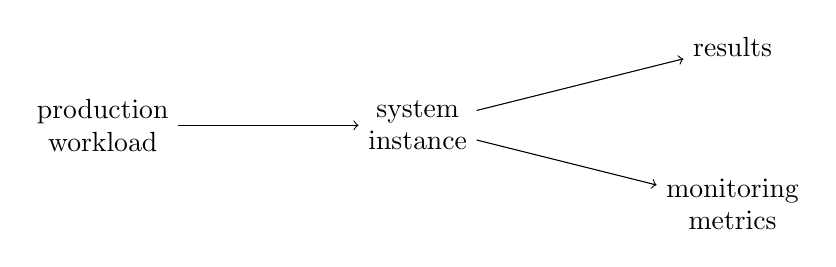
\begin{tikzpicture}[x=2cm]
                        \node (pw) at (0, 0) {\shortstack{production\\workload}};
                        \node (si) at (2, 0) {\shortstack{system\\instance}};
                        \node (r) at (4, 1) {results};
                        \node (mm) at (4, -1) {\shortstack{monitoring\\metrics}};

                        \draw
                        (pw) edge [->] (si)
                        (si) edge [->] (r)
                        (si) edge [->] (mm);
                    \end{tikzpicture}
                \end{center}
                The alternative is \textbf{benchmarking}, which is measuring in the lab.
                Since some systems run continuously, they can store state, therefore the first step in benchmarking is to put the system into a \textbf{pre-defined / steady state}, which is reasonably close to what a system would be in production.
                After this, a series of operations (the workload) is performed with relevant metrics measured.
                For example, to benchmark a database system, some data is typically generated and loaded to put the system into a steady state, and a query set is run (which we actually measure metrics for).
                \begin{center}
                    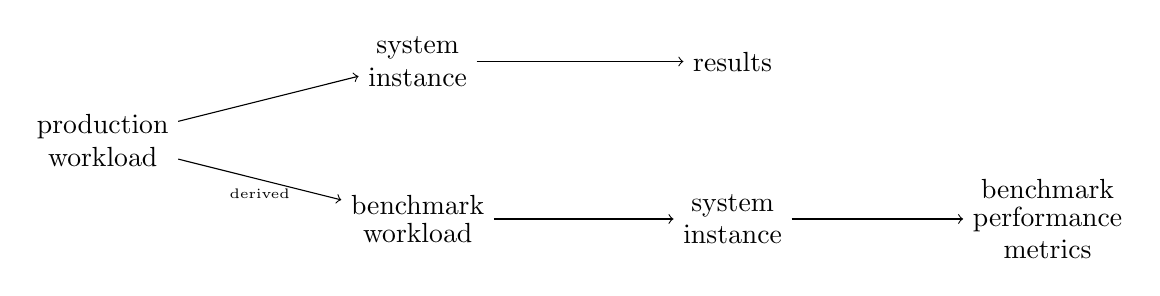
\begin{tikzpicture}[x=2cm]
                        \node (pw) at (0, 0) {\shortstack{production\\workload}};
                        \node (si1) at (2, 1) {\shortstack{system\\instance}};
                        \node (r) at (4, 1) {results};
                        \node (bw) at (2, -1) {\shortstack{benchmark\\workload}};
                        \node (si2) at (4, -1) {\shortstack{system\\instance}};
                        \node (bmm) at (6, -1) {\shortstack{benchmark\\performance\\metrics}};

                        \draw
                        (pw) edge [->] (si1)
                        (pw) edge [->, below] node{\tiny derived} (bw)
                        (si1) edge [->] (r)
                        (bw) edge [->] (si2)
                        (si2) edge [->] (bmm);
                    \end{tikzpicture}
                \end{center}
                % CONTINUE AT 1:19:39
                % nvm I'm not doing this module anymore.
\end{document}